\subsection{Accuracy convergence}
In this section we are going to investigate how the accuracy of our prediction converges as the size of the data increases.
All tests are done using a percentage of the 1348428 for training and 577552 games are used for evaluation. in each test we use all the prematch features. The classifier used in this test is logistic regression with stochastic gradient descent with L2 regularization and a ridge value of 0.01. The size of the training set used are as follows: 
\begin{enumerate}
\item 6\%: 84529 matches
\item 12.5\%: 168431 matches 
\item 25\%: 337146 matches 
\item 50\%: 674438 matches
\item 100\%: 1348428 matches 
\end{enumerate}
% Graph for big data testing. 
\begin{figure}[!htb]
  \centering
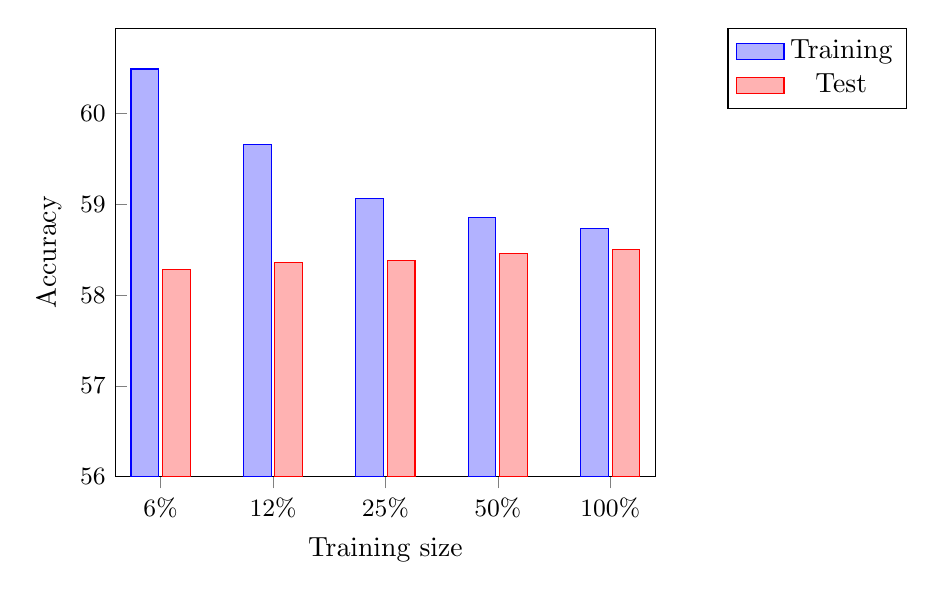
\begin{tikzpicture}
\begin{axis}[
    ybar,
    ylabel = Accuracy,
    xlabel = Training size,
    tick label style={font=\small},
    tickpos=left,
    xticklabels={6\%, 12\%, 25\%, 50\%, 100\%}, 
    xtick={1,2,3,4,5, 6},
    ymin=56,
    legend entries={Training,Test},
    legend style={at={(1.3,1.0)},
        anchor=north,legend columns=1
    },
    legend image code/.code={%
      \draw[#1] (0cm,-0.1cm) rectangle (0.6cm,0.1cm);
    }   
    ]   
    \addplot +[bar shift=-.2cm] coordinates {(1,60.49) (2,59.66) (3,59.06)  (4,58.85)     (5,58.73)  };

    \addplot  +[bar shift=.2cm]coordinates {(1,58.28) (2,58.36) (3,58.38) (4,  58.46) (5,58.50) };

\end{axis}
\end{tikzpicture}
  \caption{Test for representation of features}\label{fig:clusterbigdata}
\end{figure}
The results from \Cref{fig:clusterbigdata} shows that as more data is used to train the model the prediction accuracy on the test set increases the total change from 84529 matches to 134828 matches is $3.86\times10^{-1}\%$

The results also shows the as the size of the training data increases overfitting decreases. The difference in accuracy between the training set and test set moves from $3.79\%$ for $84529$ matches to $3.79\times10^{-1} \%$ for $1348428$ matches. The result shows that the model do not improve a lot as the amount of data increases. The test shows that as the amount of data used for training increases overfitting decreases.      
\subsubsection{Big data improvements}
To test if big data gives an improvement when predicting the outcome of a match, the same features and method where used on an increasing sized data starting from 1000 matches. After the model was made, it was tested on the training data, as a $\frac{2}{3}$-split and finally cross-validation. And as seen on \Cref{fig:bigdata} there will be more information once more tests has been run!

\begin{figure}[!htb]
  \centering
  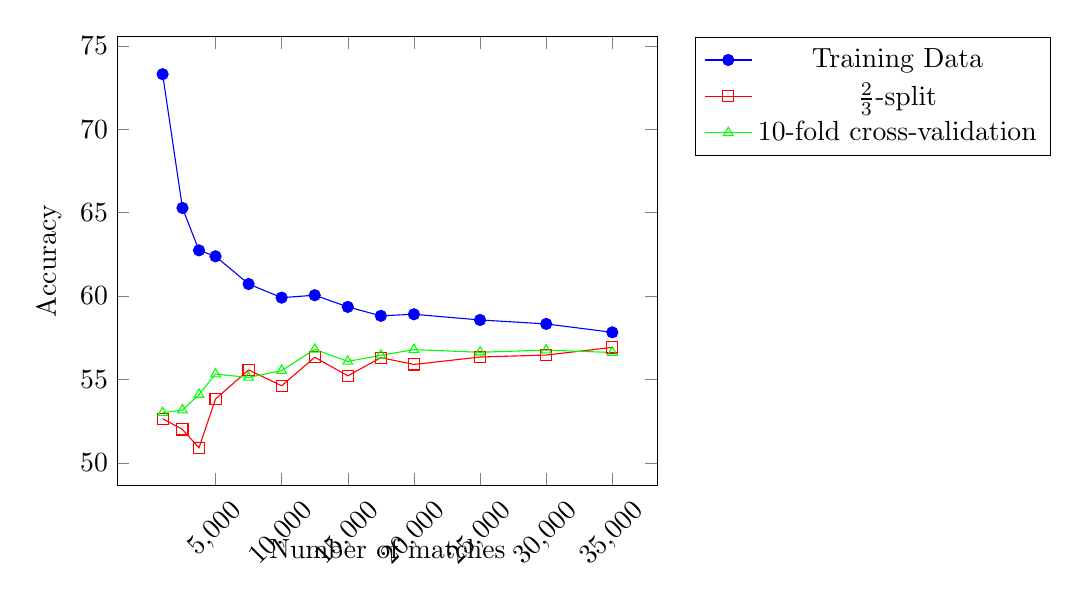
\begin{tikzpicture}[] 
    \begin{axis}[
      xlabel=Number of matches, 
      ylabel=Accuracy,
      xtick={5000,10000,15000,20000,25000,30000,35000},
      xticklabel style={rotate=45,anchor=near xticklabel},
      scaled x ticks=false,
      x label style={at={(axis description cs:0.5,-0.1)},anchor=north},
      legend style={at={(1.4,1.0)},
        anchor=north,legend columns=1},] 
      \addplot[color=blue,mark=*] coordinates {
        (1000, 73.3)    
        (2500,65.28)    
        (3750,62.7367)  
        (5000,62.38)
        (7500,60.72)
        (10000,59.9)
        (12500,60.048)
        (15000,59.3467)
        (17500,58.8114)
        (20000,58.905)
        (25000,58.564)
        (30000,58.3267)
        (35000,57.8229)
      };
      \addplot[color=red,mark=square] coordinates {
        (1000,52.6471)
        (2500,52)
        (3750,50.902)
        (5000,53.8235)
        (7500,55.5686)
        (10000,54.6176)
        (12500,56.3294)
        (15000,55.2157)
        (17500,56.3025)
        (20000,55.8971)
        (25000,56.3412)
        (30000,56.4608)
        (35000,56.916)
      };
      \addplot[color=green,mark=triangle] coordinates {
        (1000,53)
        (2500,53.16)
        (3750,54.0944)
        (5000,55.32)
        (7500,55.12)
        (10000,55.53)
        (12500,56.8)
        (15000,56.08)
        (17500,56.4457)
        (20000,56.785)
        (25000,56.628)
        (30000,56.7567)
        (35000,56.6143)
      };
      \legend{Training Data, $\frac{2}{3}$-split, 10-fold cross-validation}
    \end{axis} 
  \end{tikzpicture}
  \caption{Test for representation of features}\label{fig:bigdata}
\end{figure}
